\chapter{Array Implementation} % Write in your own chapter title
\label{Chapter4}
\lhead{Chapter 4. \emph{Array Implementation}} % Write in your own chapter title to set the page header
\section{Methodology}
Quadratic Probing for Hash tables is used to carryout basic operations on the data array. These basic operations and their working are as follows:

\subsection{Insertion}
First of all an array of size of data is created. The data is inserted at the given index and that cell is marked as legitimate.

Time Complexity: \textbf{O(1)} \\
Space Complexity: \textbf{O(N)}

\subsection{Finding}
In order to find the data, the array is traversed until our required key is found and the index of that cell is returned.

Time Complexity: \textbf{O(N)} \\
Space Complexity: \textbf{O(N)}

\subsection{Sorted Traversal}
For sorted traversal, the array is sorted using quick sort algorithm and then it is traversed to print the data.

Sorting Algorithm Used: \textbf{Quick Sort O(log N)} \\
Time Complexity: \textbf{O(N log N)}\\ 
Space Complexity: \textbf{O(N)} \\

\subsection{Deletion}
Deletion is carried out by finding the cell in which the id to be deleted is present, then the cell is marked as deleted. 

Time Complexity: \textbf{O(1)} \\
Space Complexity: \textbf{O(N)}


\section{Execution Times and Memory Consumptions}
\begin{figure}[H]
	\centering
	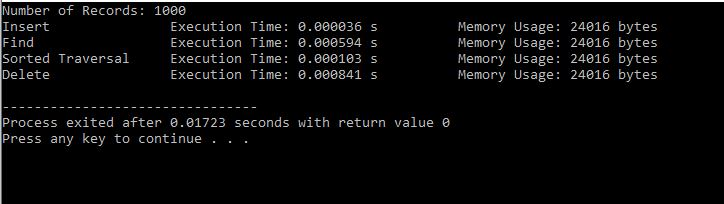
\includegraphics[scale =0.7]{./Figures/Array1000.jpg}
	\rule{35em}{0.5pt}
	\caption{Results for array implementation with data size 1000.}
	\label{fig:Array 1000}
\end{figure}

\begin{figure}[H]
	\centering
	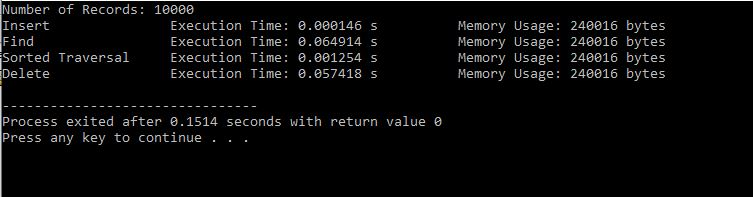
\includegraphics[scale =0.7]{./Figures/Array10000.jpg}
	\rule{35em}{0.5pt}
	\caption{Results for array implementation with data size 10000.}
	\label{fig:Array 10000}
\end{figure}

\begin{figure}[H]
	\centering
	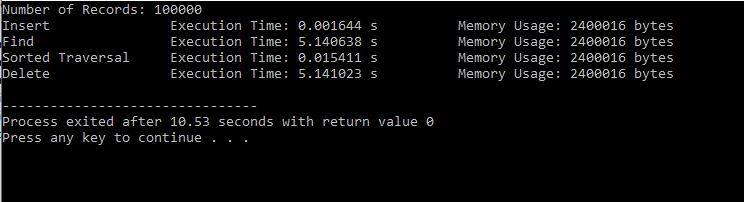
\includegraphics[scale =0.7]{./Figures/Array100000.jpg}
	\rule{35em}{0.5pt}
	\caption{Results for array implementation with data size 100000.}
	\label{fig:Array 100000}
\end{figure}

\begin{figure}[H]
	\centering
	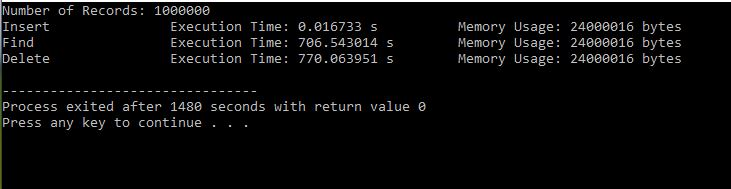
\includegraphics[scale =0.7]{./Figures/Array1000000.jpg}
	\rule{35em}{0.5pt}
	\caption{Results for array implementation with data size 1000000.}
	\label{fig:Array 1000000}
\end{figure}
